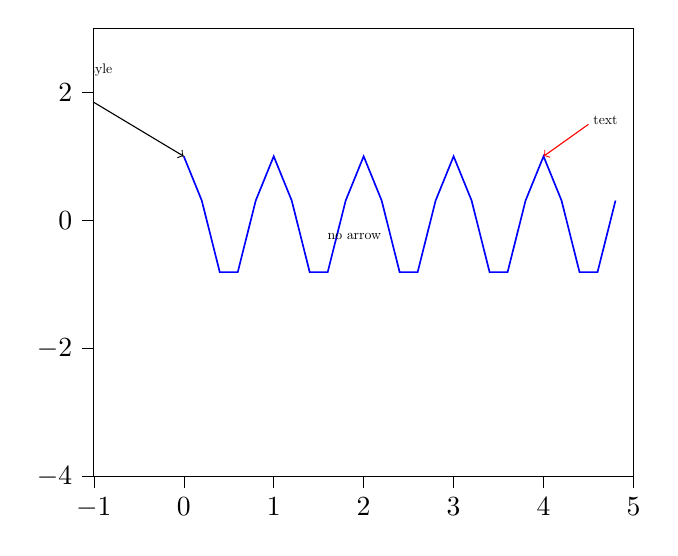
\begin{tikzpicture}

\begin{axis}[
tick align=outside,
tick pos=left,
x grid style={white!69.01960784313725!black},
xmin=-1, xmax=5,
xtick style={color=black},
y grid style={white!69.01960784313725!black},
ymin=-4, ymax=3,
ytick style={color=black}
]
\addplot [semithick, blue]
table {%
0 1
0.2 0.309016994374947
0.4 -0.809016994374947
0.6 -0.809016994374947
0.8 0.309016994374947
1 1
1.2 0.309016994374947
1.4 -0.809016994374947
1.6 -0.809016994374948
1.8 0.309016994374947
2 1
2.2 0.309016994374946
2.4 -0.809016994374948
2.6 -0.809016994374948
2.8 0.309016994374947
3 1
3.2 0.309016994374948
3.4 -0.809016994374949
3.6 -0.809016994374948
3.8 0.309016994374947
4 1
4.2 0.309016994374948
4.4 -0.809016994374949
4.6 -0.809016994374946
4.8 0.30901699437495
};
\draw[->,red] (axis cs:4.5,1.5) -- (axis cs:4,1);
\draw (axis cs:4.5,1.5) node[
  scale=0.5,
  anchor=base west,
  text=black,
  rotate=0.0
]{text};
\draw[->,black] (axis cs:0,1) ++(-50pt,30pt) -- (axis cs:0,1);
\draw (axis cs:0,1) ++(-50pt,30pt) node[
  scale=0.5,
  anchor=base west,
  text=black,
  rotate=0.0
]{arrowstyle};
\draw (axis cs:0,1) ++(50px,-30px) node[
  scale=0.5,
  anchor=base west,
  text=black,
  rotate=0.0
]{no arrow};
\end{axis}

\end{tikzpicture}
